% *********************************************************************
% © 2021 Jeremy Sylvestre
%
% Permission is granted to copy, distribute and/or modify this document
% under the terms of the GNU Free Documentation License, Version 1.3 or
% any later version published by the Free Software Foundation; with no
% Invariant Sections, no Front-Cover Texts, and no Back-Cover Texts. A
% copy of the license is included in the appendix entitled “GNU Free
% Documentation License” that appears in the output document of this
% PreTeXt source code. All trademarks™ are the registered® marks of
% their respective owners.
%
% *********************************************************************


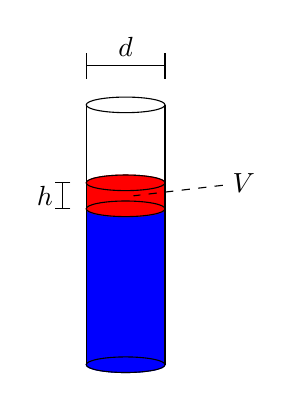
\begin{tikzpicture}[yscale=0.66]

	\draw[blue,fill] (0,0) ellipse (0.5cm and 0.15cm);
	\draw[blue,fill] (-0.5,0) rectangle (0.5,3);
	\draw[red,fill] (-0.5,3) rectangle (0.5,3.5);
	\draw[red,fill] (0,3) ellipse (0.5cm and 0.15cm);
	\draw[red,fill] (0,3.5) ellipse (0.5cm and 0.15cm);
	\foreach \y in {0,3,3.5,5} {
		\draw (0,\y) ellipse (0.5cm and 0.15cm);
	}
	\draw (-0.5,0) -- (-0.5,5);
	\draw (0.5,0) -- (0.5,5);
	\foreach \x in {-0.5,0.5} {
		\draw (\x,5.5) -- (\x,6);
	}
	\draw (-0.5,5.75) -- node[above] {$d$} (0.5,5.75);
	\foreach \y in {3,3.5} {
		\draw (-0.7,\y) -- (-0.9,\y);
	}
	\draw (-0.8,3) -- (-0.8,3.5);
	\node[left] at (-0.8,3.25) {$\change{h}$};
	\node at (1.5,3.5) (V) {$\change{V}$};
	\draw[thin,dashed] (V) -- (0.1,3.25);

\end{tikzpicture}
